\chapter{Analyse der Ausgangssituation}\label{cha:ausgangssituation}
In diesem Kapitel geht es um die Anwendung des Modulsystems auf die Renew Applikation. Dabei soll die Umsetzung der Theoretischen Konzepte innerhalb der Applikation, die sich Langfristig bewährt hat, unverändert bleiben und darüber hinaus mit den Modulsystem Eigenschaften ausgestattet werden. \bigbreak

Die initiale Entwicklung von Renew begann mit einer monolithischen Architektur. Diese erfüllte die nötigen Anforderungen, eignet sich jedoch nicht für Entwickler mit geringer Kenntnis über die Gesamtarchitektur und den darunterliegenden theoretischen Konzepten. Daher wurde eine Plugin-Architektur aufgesetzt, die es ermöglichte Studenten Renew mit Logik innerhalb eines Plugins zu erweitern. Dieses Verfahren trägt bereits den Gedanken der \textit{Modularisierung} in sich, da die Gesamtarchitektur in Bestandsteile zerlegt und mit einander entkoppelt verknüpft wird. Somit ist die Einführung des Modulsystems der nächste Schritt in Richtung erweiterbare und zusammensetzbare Systeme vorgenommen. \bigbreak

Dieses Kapitel diskutiert die Motivation für die Abschlussarbeit, setzt klare Ziele und Rahmenbedingungen und erörtert den Einfluss des Java Modulsystems auf Renew sowie die derzeitige Plugin-Architektur. Des Weiteren wird ein Zustand ermittelt, der als Basis für die nachfolgenden Prototypen gelten wird.

\section{Anforderungsanalyse} 
% Anforderungsanalyse bezieht sich auf die gesamte Arbeit und alle wesentliche Punkte
%  die in der Zukunft mit modularisierten Software-Komponenten arbeiten wird,
	Das Ziel dieser Abschlussarbeit ist die Untersuchung der Anforderungen der modularisierten Java Plattform, sowie der entsprechende Aufwand für das Anpassen bestehender Systeme. \bigbreak
	Indem der Java-JDK mit der neunten Version von Java modularisiert wurde, ändern sich grundsätzlichen Funktionsrichtlinien der Plattform, die Konsequenzen für bestehende Systeme mit sich bringen. Denn das Modulsystem von Java führt eine obligatorische Kapselung der Code-Komponenten ein, die über erweiterte Sicherheitsmechanismen verfügen und nur über explizite Schnittstellen geladen und angesprochen werden können.\newline 
	Nichtsdestotrotz bietet Java eine Übergangsphase an, die einen parallelen sowie zusammengesetzten Betrieb bestehender als auch neu entstandener Software verspricht.\bigbreak

	Da die Migration bestehender Systeme nicht in einem Schritt durchgeführt werden kann, müssen Kriterien für die Charakterisierung und Implementation der Module formuliert werden, um bestehende Systemelemente innerhalb einer ausgereiften Software als Module umzusetzen. Die saubere Umsetzung behandelt den internen Aufbau, Namen- und Paketkonventionen sowie die Modulschnittstellen, die das Interagieren mit den Modulen einheitlich beschreiben und einen Vertrag mit den Nutzer eingehen. Zusätzlich muss der Inhalt eines Moduls klar festgelegt werden, da dieser nur einen Teil der zusammengesetzte Software abbildet und den Umfang eines Moduls beschränkt.  \bigbreak 

	Jede kleine Änderung in einem komplexen System bringt große Risiken mit sich, die das sauberen Arbeit der Software wird in Frage gestellt. Es müssen neue Konzepte integriert, Richtlinien befolgt und veraltete Konstrukte ersetze werde. Zu den genannten Problemen gehören Zyklen, Split-Packages und interne API-Zugriffe, die für den Umstieg sorgfältig gepflegt werden müssen. Daher ist der Übergang auf das Modulsystem von Java mit Unsicherheit verbunden, zumal dieses Zeit kostet, im Code verankertes Geschäftswissen umstrukturiert und keine sichtbare Softwareerweiterung für den Endkunden darstellt. \newline
	Demnach liegen die Schwerpunkte der Migration in der Konsistenz der gegebenen Software im neuem Kontext sowie in dem Aufwand der Umsetzung. 
	\bigbreak

	Um die gegebenen Anforderungen an eine Applikation zu stellen bedarf es eine passende Projektstruktur und Umsetzungswerkzeuge, die eine Modulmenge kompilieren und verpacken. Zu diesen Zweck wird das Gradle Werkzeug eingeführt, das eine kompakte und mächtige Ausdrucksform für das Erstellern von Java Applikationen Entwicklungsumgebung unabhängig anbietet. \bigbreak

	Für die Umsetzung der erarbeiteten Konzepte steht der Renew Simulator und das Mulan Rahmenwerk zur Verfügung, die in dieser Abschlussarbeit  Migrationsszenarien erleben. Das erste Szenario soll eine kontinuierliche Migration einer Software auf das Modulsystem modellieren. Im Gegensatz dazu, wird im zweiten Szenario nicht modularisierte Software auf die modularisierte Code-Basis aufgesetzt und der parallele Betrieb begutachtet.  

\section{Anforderungsspezifikation} % ansich sind das die rahmenbedingunen a
	% was sind keine Ziele 
	% Gradle wollte Modl haben es kommt hier rein 
	Für den Anwendungskontext der Modularisierung einer größeren Anwendung steht Renew und Mulan zur Verfügung, jedoch übersteigern die gelistete Aufgabenmenge  aus der Anforderungsanalyse den Zeitrahmen dieser Abschlussarbeit, da die Umstellung jedes einzelne Plugins auf Modulverbände eine zeitintensive Aufgabe verkörpert. Jedes einzelne Plugin muss analysiert, auf Module zerlegt und bestens mit einander Verbunden werden. Darüber hinaus müssen die entstandenen Module mit allen anderen Plugins abgestimmt werden, da das Plugin Modulverband generell andere Schnittstellen anbieten wird. Dementsprechend wird die Modularisierung auf einzelne Plugins reduziert, die für die Darstellung der UI sowie die grundsätzliche darunterliegende Logik zuständige sind. Um die Kommunikation im bestehenden System zu garantieren, behalten die entstandenen modularisierten Plugins ihre Schnittstellen, damit die Funktionalität aller Plugins nicht beeinträchtigt wird und das Gesamtsystem einen nahtlosen Übergang durchläuft. Hierfür werden die Plugin Module mit den entsprechend Konfigurationsdateien erweitert und mit den notwendigen Plugins verzahnt. Demnach wird die Umsetzung nur die minimalen Anforderungen des Modulsystems realisieren und das Bereinigen der internen Umsetzung der Plugins aus der Sicht lassen, obwohl es eine wünschenswerter Schritt in Richtung der Modularisierung wäre. \newline 
	Trotz allem müssen die Plugin Projekte von Renew zusätzliche Module unterstützen und die Möglichkeit bieten Renew zu erweitern und weitere Module innerhalb eines Plugins zu erstellen. Dafür benötigen die Plugins eine neue Projektstruktur die das gewünschte Verhalten umsetzt und die empfohlene Modulorganisation unterstützt. Dieses trägt die Maven konforme Projektstruktur, die Java Klassen, Ressourcen und sonstige Artefakte nach einem standardisierten Muster verwaltet. Des Weiteren muss die Konfiguration des Projektes von den Entwicklungsumgebung gelöst werden, um den Entwickler nicht in seinem Arbeitsablauf einzuschränken und die Entwicklungsumgebung seiner Wahl zu nutzen. \newline
	Da der Renew Simulator von verschiedenen Abschlussarbeiten beleuchtet und erweitert wird, beinhaltete die Applikation verschiedene Techniken der Softwareentwicklung, wie zum Beispiel das Generieren von Java Klassen mit dem \textit{JavaCC} Compiler. Dementsprechend existieren ältere Verfahren innerhalb von Renew, die sorgfältig auf Kompatibilität mit der neuen Umgebung untersucht, migriert oder ersetzt werden müssen. \bigbreak

	Die wichtigen Szenarien für das erreichen Des gesetzten Ziels werden mit zwei Prototypen umgesetzt. Der Renew Prototyp wird eine kontinuierliche  Modularisierung der Plugins und dessen Betriebsfähigkeit mit nur zum Teil Modularisierter Codebasis abdecken. Im Gegensatz dazu behandelt der Mulan Prototyp die Integration bestehender Systeme auf die Modularisierte Code-Basis. 


	% Gradle wollte Modl haben es kommt hier rein 
% Vorgehensweise 
% Einsatzszenarios und angestrebte Verbesserungen
% Funktionale Anfoderungen 
% Nicht Funktionale Anforderungen 
% Rahmenbedingungen 


\section{Motivation}\label{sec:motivation}
Es gibt mehrere Gründe warum Renew die Migration auf das Modulsystem durchführen sollte. Im Folgenden werden die wesentlichen Gründe, die für die Migration sprechen diskutiert.  

\subsection{Verkürzter Entwicklungszyklus}\label{sub:vez}
Die Aufteilung einer monolithischen Architektur auf eine Plugin-Architektur war ein großes Ereignis für Renew. Denn mit der Zerlegung der Gesamtarchitektur, wurde die Komplexität auf die entstandenen Komponenten aufgeteilt und erlaubte eine mühelose Weiterentwicklung der Applikation über die Plugins. \bigbreak

Obwohl die Renew Plugin-Architektur lange im Betrieb blieb, hatte das Plugin-System die Codebasis umorganisiert, ohne diese zu verändern. Diese führt zu altem, unverständlichem Code aus der Java 1.4 (2002) Version, mit dem viele Konzepte und Architektur Entscheidungen getroffen wurden. Nach fast 18 Jahren Betrieb altert die Codebasis sowie die Ideen und Konzepte für die Umsetzung ihrer Funktionalität. Besonders konfus und aufgebläht können Funktionsumsetzungen erscheinen, die heute von Java 12 in ein paar Zeilen gelöst werden können. Der zügige und rapide Wandel der Software Paradigmen und deren optimaler Einsatz in der Software Architektur ist ein Teil des Fortschritts und muss in die Planung des Lebenszyklus der Applikation mit einkalkuliert werden. \newline

Daher ist die Modularisierung und dessen Anforderung an die Struktur und Inhalt ein wichtiges Ereignis für den Renew Lebenszyklus. Denn dieser erreicht wieder sein Ende und wird mit dem Modularisierungsschritt zurückgesetzt. \bigbreak

Renew's Entwicklungseinheit ist das Plugin. Diese repräsentiert ein bestimmtes Feature mit einem eigenen Lebenszyklus, wie zum Beispiel ein Formalismus, Simulator oder Fenster Management Plugin. Diese müssen Daten entgegennehmen, diese verarbeiten und wieder ausgeben. Demzufolge bündelt ein Plugin mehrere Fähigkeiten, die zusammen ein Feature verkörpern. Somit können Codeänderungen an mehreren Stellen im Plugin das Verhalten des Plugins beeinträchtigen und müssen auf das Gesamtverhalten des Plugins und seiner Nutzer getestet werden. Mit der Einführung der Module, kann das Plugin in kleinere Einheiten zerlegt werden, die anschließend eine gekapselte Teilfunktionalität des Plugins in sich tragen und Auswirkungen der Modifikation eingrenzen. Diese sind klein, leicht änderbar, ersetzbar und besitzen einen eignen Lebenszyklus. Somit verkürzt sich die Entwicklungsdauer einer Änderung und bietet eine Möglichkeit kooperativ und parallel an einem Plugin zu arbeiten. \newline

Demnach erweitert die Modularisierung den Renew Kontext und erlaubt das Entwickeln von Plugins in Rahmen eines Studenten Projekts, indem Teilaufgaben eines Plugins auf Module zerlegt und parallel von Studenten bearbeitet werden können. Darüber hinaus ist das Zusammenführen der Ergebnisse eine konfliktfreie Angelegenheit und bedarf keine komplette Gruppenaufmerksamkeit, um die passenden Codeblöcke für die Gesamtfunktionalität auszuwählen, da es so gut wie keine Überschneidung in der Aufgaben Implementation sich bilden kann. Somit profitiert Renew von den kurzen Entwicklungszyklen der Module und deren unproblematischen Verknüpfungseigenschaften. 

\subsection{Code-Bausteine}\label{sub:cbs}
Eine der wichtigsten Fähigkeiten eines Entwicklers, ist die Beherrschung der Komplexität. Diese führt zu sauberem, lesbarem, wartbarem Code und erweitert den Lebenszyklus einer Software um ein Vielfaches. Um diese Kompetenz zu meistern bietet das Modulsystem von Java unterstützende Werkzeuge, die den erstellten Code organisieren und strukturieren, um ein langlebiges Ergebnis zu erzielen.  \newline

Da Renew das Produkt vieler Abschluss-, Projekt- und Doktorarbeiten ist, durch die die Software ihre Gestalt annimmt, gibt es diverse Beschäftigte mit eigenen Zielen und Interessen. Daher ist eine allgegenwärtige, globale Strukturanforderung, die jedem Entwickler bekannt ist und die verpflichtend eingehalten werden muss, eine erstrebenswerte Charakteristik.  \newline

Die im Kapitel \ref{cha:modularisierung} vorgestellten Moduleigenschaften beschreiben die von dem Java Modulsystem eingesetzten Richtlinien für die saubere Softwareentwicklung und erzwingen ein Still der fein granulierten Code-Bestandteile, die kombiniert eine Softwaresystem darstellen. \newline

An erster Stelle verhindert dieses Vorgehen den sogenannten \textit{Spaghetti Code}, der funktionsübergreifende Anpassungen trifft und den Überblick über den Zusammenhang der Gesamtarchitektur unscharf erscheinen lässt.  \newline

Module erschweren den \textit{Spaghetti Code}, indem Mehraufwand für die Kommunikation zwischen den Modulen erbracht werden muss und machen das unsaubere Arbeiten unattraktiv. Somit dienen Module als Grenzen für den Entwicklungsrahmen eines Features und engen den Bearbeitungs- und Betrachtungsraum für den Entwickler ein. Daraus ergibt sich ein Softwarepaket, das unabhängig von den Senior-Entwicklern verstanden, genutzt und angepasst werden kann, da der Aufbau nicht mehr in dem Wiki, Readme oder beim Entwickler selbst verankert, sondern direkt in der Codebasis integriert ist.  \newline

Demzufolge profitiert Renew von der Modularisierung, indem sich immerfort wechselnden Akteure eine saubere Codebasis hinterlassenen, die für den nächsten Absolventen sowie den wissenschaftlichen Mitarbeitern viel Zeit erspart. \bigbreak

Aus einer sauberen Umsetzung folgen saubere Code-Bausteine, die wiederverwendet werden können. Die genannten Eigenschaften der Module bringen einen wesentlichen Vorteil beim Optimieren der Renew Applikation, indem kontextbezogen Module ausgetauscht werden können, um ein besseres, lokales Erlebnis zu erzielen. Zum Beispiel können zielgerichtet ausgewählte Plugins für die Erfüllung einer speziellen Aufgabe, wie das Validieren von P/T-Netzen, ein besseres Ergebnis abliefern, indem ein für diesen Anwendungsfall angepasste Verarbeitungsalgorithmus angewandt wird. Dieser ist natürlich in einem Modul gekapselt und besitzt Schnittstein identisch zu seinem Vorgänger. Auf diese Weise kann eine große Anzahl an Modulen mit gleicher Funktion und unterschiedlicher Zielsetzung erstellt werden, die in einem Modulkatalog verwaltet und bei Bedarf ausgetauscht werden können.

\subsection{Vision} \label{sub:moderner_zustand}
% Ziel
Der zeitgemäße Zustand einer Applikation ist ein Zeichen hoher Qualität und reflektiert enorme Ansprüche an den Betrieb der Applikation. Diese kann geschäftskritische Qualitäten tragen, die den marktführenden Vorteil bringt und der Konkurrenz ein Schritt voraus ist. Um den Vorsprung zu sichern, ist eine \textit{vorausschauende} Flexibilität gefragt. Mithilfe dessen die Applikation in der Lage ist, mit minimalem Aufwand, an die führenden Technologien anzuknüpfen. 

% Trends 
Die aktuell führenden Trends beschäftigen sich mit der verteilten und wiederverwendbaren Softwareumsetzungen, die ständig an Komplexität gewinnen und trotzdem leicht beherrschbar bleiben muss. Diese beschreiben Ansätze wie gewisse Ziele erreicht werden können und setzen Grundvoraussetzungen zum erreiche dieser Ziele. Dementsprechend muss Renew bestimmte Grundvoraussetzungen erfüllen, um die Vorteile der Trends zu Nutzen und den Schritt mit dem Fortschritt zu halten.  \bigbreak


% Docker  
Zum Beispiel wäre die Docker Umgebung für Renew eine willkommene Erweiterung, mit der interne Bestandsteile distributiv betrieben werden können. Somit wäre die Ausführung von Renew nicht mehr an eine Maschine gebunden und kann bei Bedarf horizontal skaliert werden. Im Folgenden stellt sich die Frage: welche internen Strukturen von Renew müssen individuell behandelt und anschließend kooperativ zusammengeführt werden. Auf diese Frage gibt es keine pauschale Antwort, jedoch ist es klar, dass die Plugins von Renew Feingranular betrachtet werden müssen, um sich ein Bild der Verarbeitungskette zu erstellen und diese den Bedürfnissen anzupassen. \bigbreak

% Microservice  
Renew auf verschieden Hardwareknoten zu verteilen ist nur der erste Schritt der distributiven Ausführung. Es fehlt die Koordination zwischen den Knoten, die die Verarbeitung koordinieren und die Ergebnisse zusammenfassen. Somit gibt es eine weitere Technologie, die sich dieser Aufgabenstellung widmet: Der Mikroservice Architekturansatz, der sich um die Koordination und das Zusammenspiele von \textit{Applikationsschwärmen} kümmert. \bigbreak

% Fazit 	
Mithilfe der Mikroservicearchitektur und der Docker-Umgebung wäre die distributive Ausführung von Renew erreichbar, doch zuerst muss Renew den aktuellen Stand der Technologie entsprechen und demzufolge das Modulsystem von Java integrieren.  


\section{Auswirkung} \label{auswirkung}
	Die Folgeerscheinung der Modularisierung unterbindet zahlreiche Entwicklungsschwächen, wie \textit{Zyklen}, \textit{Split Packages} und antiquierte API's. Diese sollen mit der Migration aufgelöst, reorganisiert und nachgerüstet werden, um einen kompelierfähigen Zustand erreichen zu können.

\subsection{Zyklen Frei} 
	Mit den Zyklen freien Plugins werden Abhängigkeiten aufgelöst, die sich an falschen stellen befinden und mehr als eine Aufgabe Plugin übergreifend lösen möchten. Diese haken sich in den Betrieb der unmittelbar angrenzenden Komponenten ein und machen sich unverzichtbar für die Ausführung der Software. Die minimale Renew Version hat keine Laufzeitzyklen und erfüllt somit das Kriterium der Zyklen Freiheit, nichtsdestotrotz sind diese in der erweiterten Version nicht ausgeschlossen.

\subsection{Split Packages}
	Der Mangel der namensgleichen Pakete wird in einer Plugin-Architektur mit großer Wahrscheinlichkeit einträten, da Plugins aus dem gleichem Kontext, wie \textit{Navigator} oder \textit{NavigatorGit}, den selben \textit{de.renew.navigator.*} Namensraum beanspruchen. Dieses führt zum Fehler beim Auflösen der benötigten Klasse und verhindert das Hochfahren der Applikation. 

\subsection{Schnittstellen}
	Die \textit{plugin.cfg} beschreibt die Abhängigkeit der Module unter einander, jedoch ist diese Informantin unvollständig, denn dieser fehlt die Information über Schnittstellen des Plugins und dafür ausgelegten Pakete. Infolgedessen hat der Entwickler keine andere Möglichkeit als auf gewünschte Plugin-Funktionen direkt zu zugreifen, ohne einen festen Vertrag über die Kommunikation einzugehen. Somit kann jede Änderung und Aktualisierung innerhalb eines Plugins zum unerwarteten Verhalten seiner Nutzer führen. \newline
	Im Gegensatz zu den \textit{plugin.cfg} führt die \textit{module-info.java} eine Liste an benötigten Modulen sowie exportierten Paketen, die den Zugriff von außen einschränken. Dies erlaubt nicht nur das Verständnis der benötigten Module, sondern unterstützt den Entwickler durch klar definierte Schnittstellen, die mit dem Schlüssel \textit{exports} deklariert sind.

\subsection{Homogene Umgebung}
	Ein weit verbreitetes Problem der Softwareentwicklung, ist der Unterschied der Laufzeit- sowie Entwicklungsumgebung. Die Entwickler arbeiten auf einer bestens eingerichteten Maschine mit allen nötigen Bibliotheken und Abhängigkeit, die in der Zielumgebung zu meist nicht existieren. Um die Diskrepanz des Ausführungskontext entgegen zu wirken, wird eine Richtlinie benötigt, die den Kontext einer Applikation beschreibt. Aus diesem Grund deklariert die \textit{module-info.java} eine globale Plattformunabhängige Anforderung an benötigten Modulen und Bibliotheken, die zu der Kompilations- sowie Ausführungszeit präsent sein müssen.\bigbreak

	Die Renew \textit{plugin.cfg} erfüllt die Funktion einer Richtlinie der benötigten zugrunde liegender Plugins, jedoch fehlen die Deklaration der unterstützenden Bibliotheken, die für die Ausführung von Renew benötigt werden. Daher ist die explizite Deklaration der notwendigen Drittanbieter-Bibliotheken wie \textit{log4j} eine willkommene Erweiterung für Renew. 

\subsection{Service Loader} 
	Der Renew Plugin-Manager ist der Kern der Applikation und verbindet alle Plugins und erforderliche Drittanbieter-Bibliotheken miteinander. Die geschickte Umsetzung entkoppelt Komponenten voneinander und erlaubt das einfache hinzufügen sowie entfernen von Plugins, ohne die bestehende Architektur zu verändern. Die notwendigen Werkzeuge, die im Grundlagenkaltteil besprochen wurden, ermöglichten die Umsetzung der dynamische Plugin Kopplung. \bigbreak

	Obwohl die Plugins Unabhängig voneinander entwickelt werden können, musste die interne Funktion an die umgebenen Plugins durch direkte Zugriffe gebunden werden. Daraus folgt eine wilde Kopplung jedes einzelnen Plugins mit der umgebenden Logik. Zum Beispiel greift das \textit{Gui}-Plugin direkt auf den \textit{Formalism}- sowie den \textit{Simulator}-Plugin zu und manipuliert somit den Zustand der Applikation. Im Gegensatz dazu manipuliert das \textit{CNFormaism}-Plugin seinen Zustand direkt über das \textit{CH.if.draw}-UI-Framework. In der Konsequenz ergibt sich widersprüchliche Kontrollflüsse.\newline  
	Um die Kontrolle über alle möglichen Plugin Typen zu behalten, kann das \textit{Gui}-Plugin über den \textit{Java Service Loaders} Mechanismus alle eingebundenen \textit{Formalism}-Plugins auslesen. Dafür wird ein \textit{Formalism}-Schnittstellen Modul erstellt, welches anschließend von anderen Modulen implementiert werden kann. Zum Beispiel können die \textit{CNFormalism} und das \textit{FAFormalsim}-Plugin's, die als Module implementiert sind, mithilfe des \textit{provide with} Schlüssels eine Implementation für das \textit{Formalism}-Modul anbieten. Diese werden anschließend über die \textit{Java Servide Loader Registery} von dem \textit{Gui}-Plugin ausgelesen und verwaltet. \bigbreak

	Die Instanziierung der Plugins über das \textit{IPLugin} Interface verfolgt einen ähnlichen Ansatz und war somit seiner Zeit voraus. Jedoch hat Java aufgeholt und bietet eine leichtgewichtige und native Umsetzung des Registrierdienstes mit einer variablen Menge an möglichen Interface Implementationen von der Renew profitieren kann.   

\subsection{Plugin Manager}
% DAG der Module 
	Der \textit{Plugin Manager} ist verantwortlich für das Erfassen und Einlesen der Renew Codebasis in dem Arbeitsspeicher. Die Reihenfolge für die Plugin-Architektur ist strikt, da bestimmte Plugins gewisse Drittanbieter sowie Plugin-Bibliotheken brauchen. Wenn die Reihenfolge nicht stimmt werden benötigte Klassen nicht gefunden und die Applikation bricht mit einem Fehler ab. Daher ist das Ladend der Drittanbieter-Bibliotheken und das anschließende Laden der Plugins in der richtigen Reihenfolge eine kritische Aufgabe. \bigbreak

	Das Modulsystem von Java bringt einen neuen Abschnitt in den Lebenszyklus einer Java Applikation, der diese wichtige Aufgabe des \textit{Plugin Managers} übernimmt. Jener erstellt, vor dem Starten der Applikation, einen gerichteten Graphen aus angeforderten Modulen sowie Bibliotheken und prüfte dessen Existenz auf dem Modulpfad. Wenn diese nicht existieren wird ein \textit{java.lang.module.FindException} Fehler geworfen, anderenfalls sind alle Voraussetzungen für das Starten der Applikation erfüllt und die Applikation beginnt ihre Ausführung. \bigbreak

	Damit übernimmt das Modulsystem von Java die Erstellung der richtigen einlese Reihenfolge der Plugins als einen gerichteten azyklischen Graphen und übernimmt eine weitere interne Aufgabe.

\section{Ausgangssituation} \label{sec:ausgangssituation} 
	In diesem Abschnitt wird die Ausgangssituation für Renew sowie Mulan dargelegt, die als Grundlage für die nachfolgenden Prototypen dienen werden. 

\subsection{Renew} \label{sub:renew}
	Renew ist in mehr als 60 Plugins aufgeteilt, die für sich alleinstehende Projekte repräsentieren. Jedes Projekt besitzt eine \textit{build.xml} und wird mit dem übergeordneten Stamm \textit{build.xml} Script zusammengeführt. Die XML-Scripte werden von dem \textit{Apach Ant} Werkzeug evaluiert, kompiliert und zusammengeführt. In Folge dessen entsteht ein \textit{jar} Archiv für jedes Plugin-Projekt. Diese werden in eine bestimmte Orderstruktur für die Ausführung aufbereitet, die sich aus dem \textit{config, plugins} und \textit{libs} Verzeichnis zusammensetzt. \bigbreak

	Der innere Aufbau jedes Plugins benötigt eine besondere Konfigurationsdatei, nämlich die \textit{plugin.cfg}. Diese beschreibt für die Ausführung nötige Plugin-Abhängigkeiten und wird von dem internen Plugin-Manager verwaltet, der für die richtige Ordnung beim Laden jedes einzelnen Plugins aus dem \textit{plugins} Verzeichnis sorgt. Somit sind die \textit{plugin.cfg} Dokumente ein guter Startpunkt für die Evaluation einer minimalen und lauffähigen Renew Konfiguration. \bigbreak

	\begin{figure}[h!]
	  \centering
	  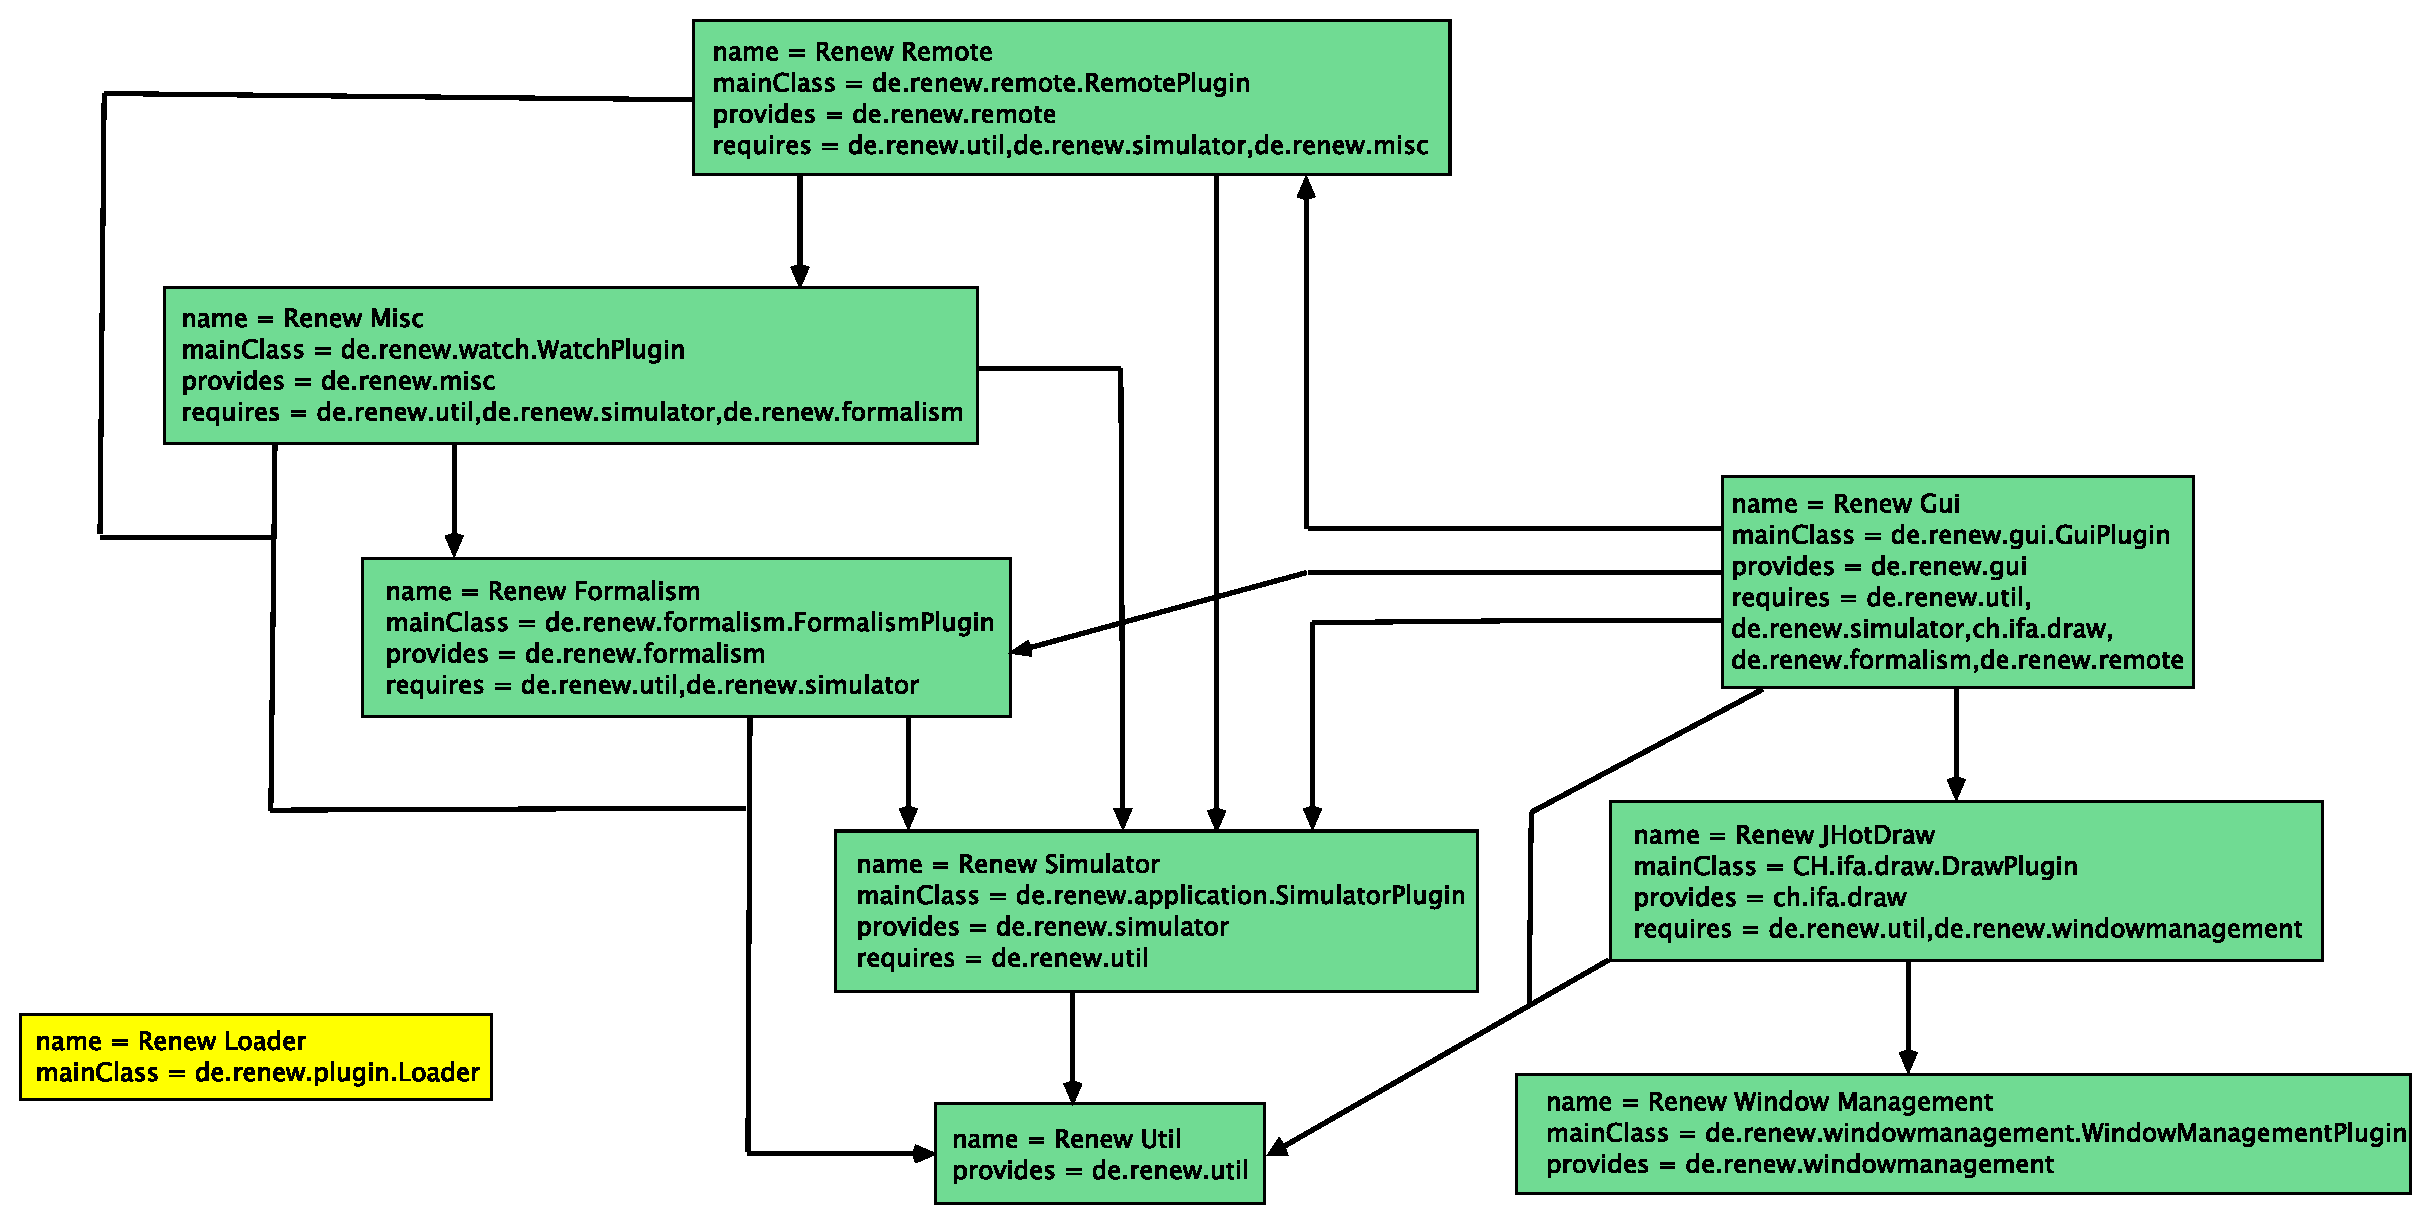
\includegraphics[width=\textwidth]{material/images/renew_plugin_dependencies2.pdf}
	  \caption{Gui Plugin-Abhängigkeiten}
	  \label{fig:plugin_deps}
	\end{figure}

	Für die Evaluation der minimalen Konfiguration starten wir aus dem \textit{Gui}-Plugin und arbeiten uns abwärts der Plugin-Hierarchie der \textit{plugin.cfg} hinab, bis der komplette Graph aufgebaut ist.\newline

	Die in der Abbildung \ref{fig:plugin_deps} repräsentierten Zusammenhängen reflektieren die von den Entwicklern abgestimmten Laufzeitabhängigkeiten, die einen groben Überblick über die nötigen Plugins verschaffen. Diese können zur Laufzeit alle benötigten Daten und Klassen enthalten, jedoch tragen sie keine Aussage über Abhängigkeiten während der Kompilation. Demgemäß kann zusätzlicher Code sowie Plugins benötigt werden. 


\subsection{Mulan} \label{sub:mulan}
	Mulan \cite{Roelke04} ist ein Multiagenten Rahmenwerk, mit dem Agenten entwickelt und mit einander verbunden werden können. Diese agieren nach eigenem Interesse und verhandeln über Kommunikationskanäle, die von Mulan angeboten werden. Um eine auf Mulan basierende Multi-Agent-Anwendung zu erstellen, müssen zahlreiche Protokollnetze gezeichnet und Wissensbasen erstellt werden, die das Verhalten und die Interaktion von Agenten implementieren. Somit bietet Mulan ein Kommunikationsplattform sowie ein Gerüst für die Umsetzung der darauf aufsetzenden Agenten und dessen Eigenschaften sowie Fähigkeiten, die mit Referenznetzen entworfen werden können. \cite{cabac} \bigbreak

	\begin{figure}[h!]
	  \centering
	  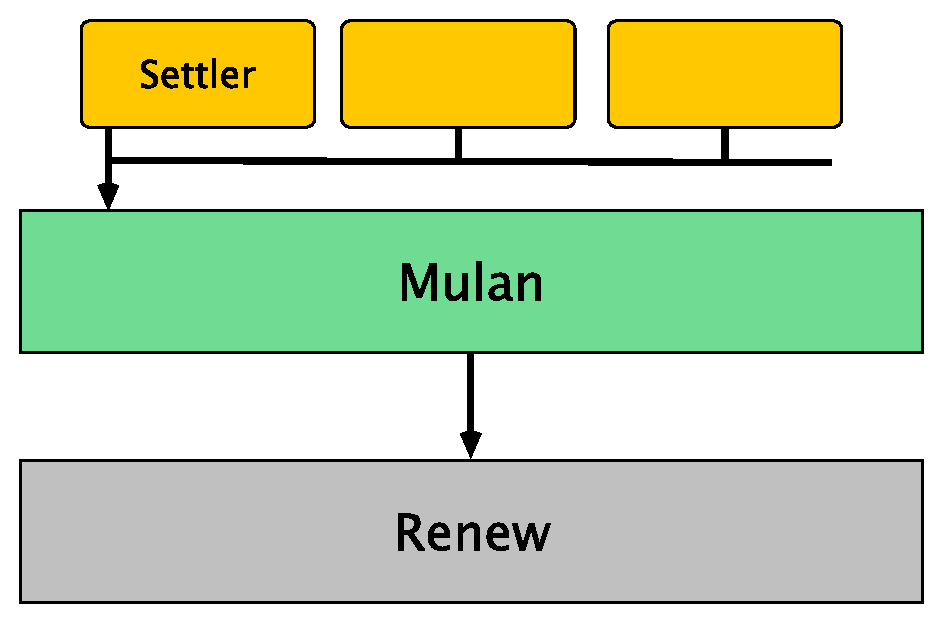
\includegraphics[width=0.5\textwidth]{material/images/settler-mulan-renew.pdf}
	  \caption{Mulan Plugins}
	  \label{fig:mulan_plugin}
	\end{figure}

	Das Spiel Settler ist mit Mulan umgesetzt und implementiert somit die Agenten Anforderungen des Multi Agenten System. Diese halten Wissensbasen über die Spielregeln und können mit Hilfe der Protokollnetze bestimmte Entscheidungen treffen und Handlungen ausführen. Wie zum Beispiel Straßen bauen oder Karten handeln.\newline
	Damit die erstellten Settler Agenten und dessen Aufbau simuliert werden kann, wird der Renew Petrinetz Simulator verwendet, mit dem die umgesetzten Agenten-Strukturen betrieben werden können.\newline
	Des weiteren besitzt das Settler Spiel sowie das Mulan-Rahmenwerk eine Plugin konforme Architektur und werden somit genauso, wie die Renew Plugins von dem Renew Plugin-Manager ausgelesen und verwaltete.\bigbreak

	Eine vereinfachter Zusammenhang ist in der Abbildung \ref{fig:mulan_plugin} dargestellt und visualisiert die benötigten Grundlagen für die Ausführung von Settler.

\section{Durchführung}
